% Условная компиляция для самостоятельной работы
\ifdefined\mainfile
    % Если это часть основного файла, не добавляем начало и конец документа
\else
    \documentclass[12pt, a4paper]{report}
    \usepackage{/Users/vladbelousov/Desktop/Semestr_4-FP-NSU/Настройка/library}
    \usepackage[utf8]{inputenc} % Подключение поддержки UTF-8
    \begin{document}
\fi

%%-------------------------------%%

\section{Линза как Фурье-анализатор}

Интеграл Киргхгофа для плоских экранов \( \displaystyle  E_p (x_p , y_p , z_p ) = \frac{k}{ 2 \pi i } \iint dx dy E(x, y , 0 ) \frac{e^{ i k R } }{R } \cos  \theta  ,    \) \( \text{где } \theta = \widehat{\vec{R }  ,\vec{n } }  \) 

Рассмотрим следующий эксперимент: 

\begin{center}
    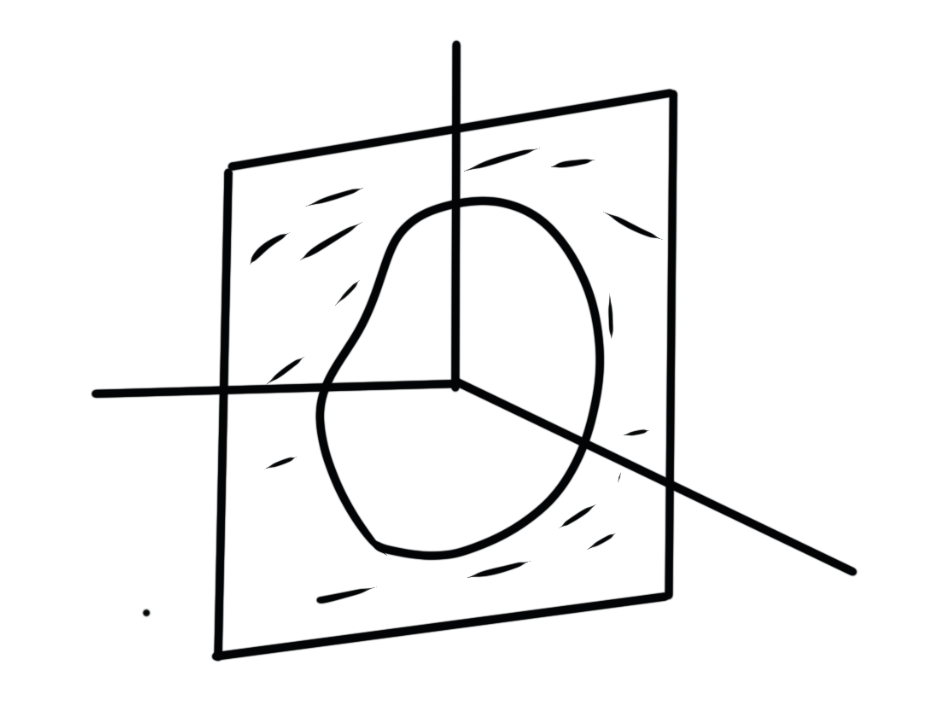
\includegraphics[width=0.4\textwidth]{/Users/vladbelousov/Desktop/Semestr_4-FP-NSU/ЭиО/Лекции_по_дням/image/171.png}
\end{center}
\( S \) - точечный источник монохроматической волны; трафарет с коэффициентом пропускания \( \tau (x,y ) \).

\[\text{В ОП}_1 :   E_1(\text{после трафарета} )= E_0 e^{ i k \left(  \left\lvert a  \right\rvert - \frac{ x_l ^2 + y_l ^2 }{2 a }  \right) \tau (x_l , y_l)}  \] 
, где \( E_0 = \displaystyle  \frac{\Delta}{R_1 } , \text{ }  R_1 = \sqrt{a ^2 + x_l ^2 + y_l ^2 } = \left\lvert  a  \right\rvert + \frac{ x_l ^2 + y_l ^2 }{2 \left\lvert a \right\rvert}  \) 

\[ \text{В ОП}_2 : E_2 = E_1 e^{ i \varphi_0 -   ik\frac{ x_l ^2 + y_l ^2       }{2 F_{\text{л} } } }; \quad  R_2 = \sqrt{b ^2 + (x_p - x_l ) ^2 + ( y_p - y_l ) ^2 } \approx b + \frac{ (x_p - x_l ) ^2 + (y_p - y_l ) ^2 }{2 b}       \] 

\[ E_p (x_p, y_p ,b ) = \frac{k}{2 \pi i } \iint d x_l d y_l E_2 \frac{ e ^{ ik R_2 } }{R_2 } \cos  \theta \approx \frac{k}{2 \pi i b } \iint d x_l d y_l E_2 e^{i k \left( b + \frac{ (x_p - x_l ) ^2 + ( y_p - y_l ) ^2 }{2 b}  \right)} =       \] 
\[ = \frac{E_0k}{2 \pi i b } \int   d x_l e^{ ik \left[ - \frac{ x_l ^2 }{2 a } - \frac{ x_l ^2 }{2 F_{\text{л} } }  + \frac{x_p ^2 - 2 x_p x_l + x_l ^2 }{2 b }    \right]} \int d y_l e ^{ ...} \tau(x_l , y_l)  \cdot e^{ ik \cdot \mathrm{const}  }  \]  

Пусть  \( \displaystyle  \frac{1}{a }  + \frac{1}{F_{\text{л} } } = \frac{1}{b}   \) (сопряженные плоскости) 

\[ E_p = \frac{ k E_0 }{2 \pi i b } \cdot e^{ ik \left[ \left\lvert a  \right\rvert  + b  \frac{ x_p ^2 + y_p ^2  }{2 b } \right] + i \varphi_0} \iint d x_l d y_l \tau(x_l , y_l) e^{ - ik \frac{ x_p x_l }{b } } e^{- ik \frac{ y_p y_l }{b} } = \frac{k E_0 }{ i b } e^{ ik \left[ \left\lvert a  \right\rvert + R_p  \right] + i \varphi_0 } \hat{ \tau } (k_x , k_y)        \] 
, где \( k_x = \displaystyle \frac{k x_p }{b } , \text{ }  k_y = \frac{ k y_p }{b}   \) 

\[ I_p = \frac{ \left\lvert E_p      \right\rvert ^2 }{2 } = \frac{ k ^2 }{ b ^2 } I_0 \left\lvert  \hat{\tau } (k_x , k_y )  \right\rvert ^2   \] 

Частный случай: \( a \to  -\infty  \Rightarrow b = F_{\text{л} }  \) 

\begin{center}
    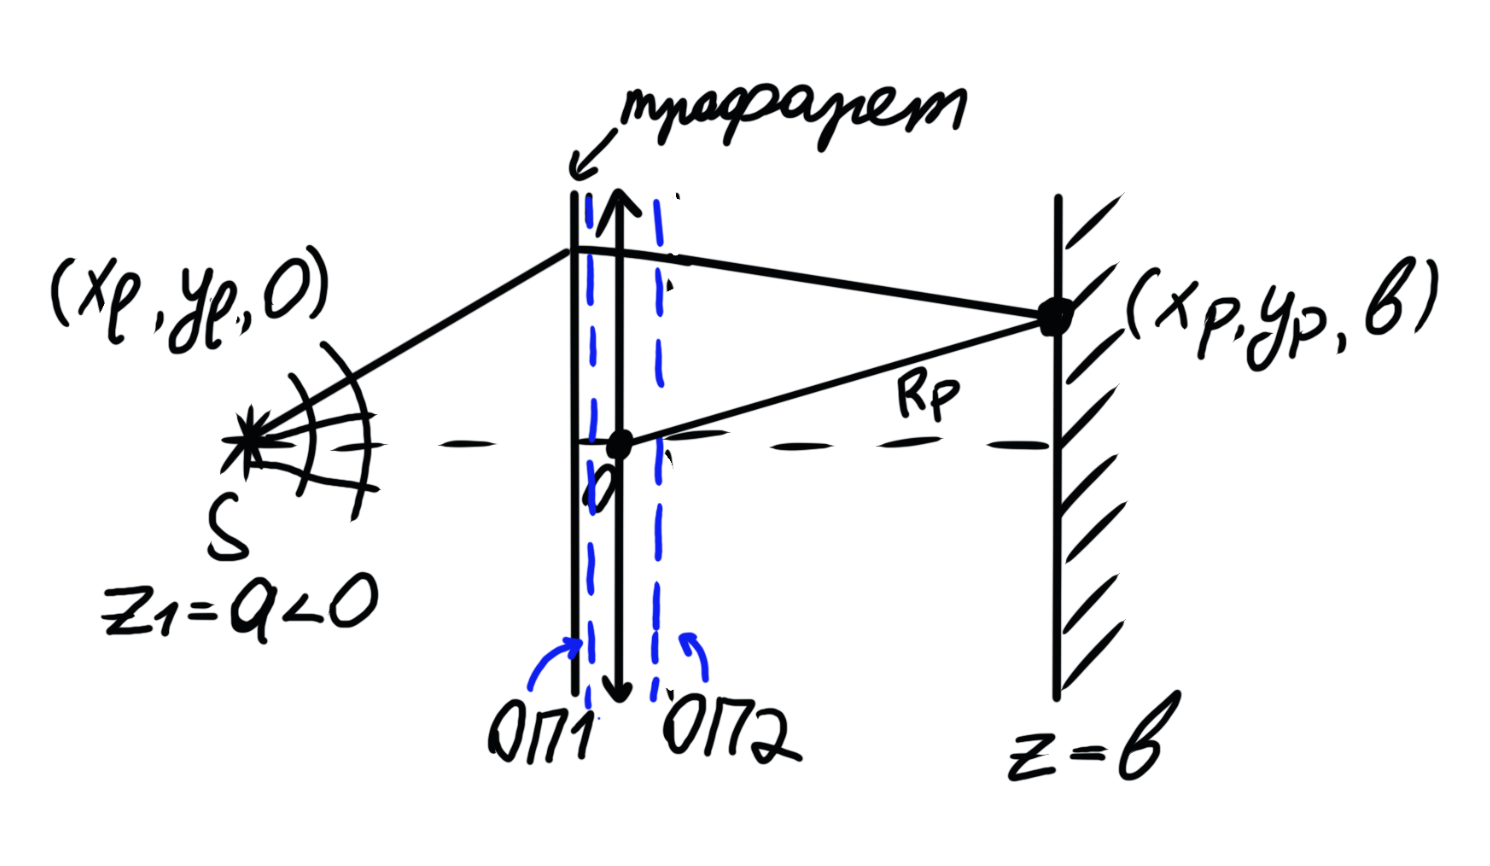
\includegraphics[width=0.7\textwidth]{/Users/vladbelousov/Desktop/Semestr_4-FP-NSU/ЭиО/Лекции_по_дням/image/172.png}
\end{center}

Рассмотрим плоской полны на трафарете, а изображение строим в фокальной плоскости линзы:

\begin{center}
    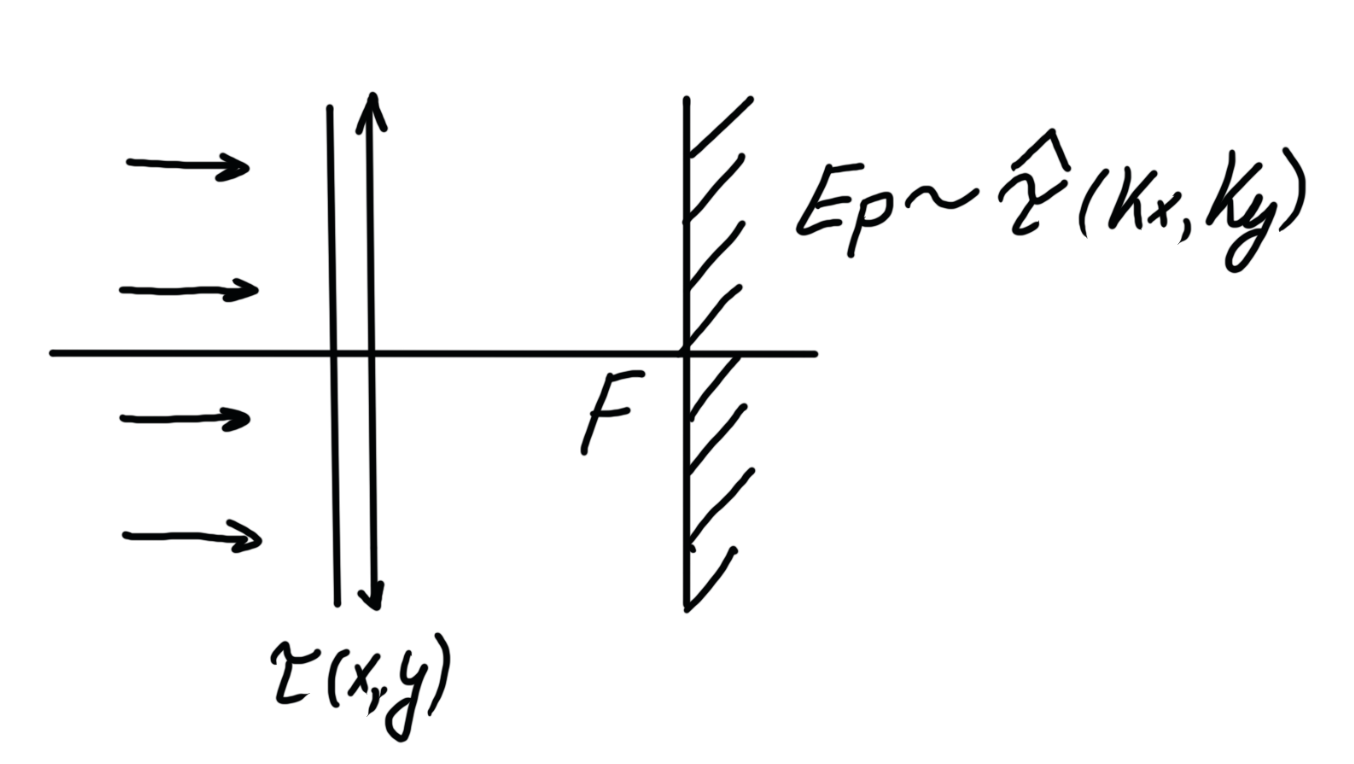
\includegraphics[width=0.5\textwidth]{/Users/vladbelousov/Desktop/Semestr_4-FP-NSU/ЭиО/Лекции_по_дням/image/173.png}
\end{center}

\[ R_1 = \sqrt{a ^2 + (x_s -x_l  ) ^2 + (y_s - y_l ) ^2 } \approx \left\lvert a  \right\rvert \frac{(x_s - x_l ) ^2 + ( y_s - y_l ) ^2 }{ 2(-a )}  \] 
\[ R_2 = \sqrt{F ^2 + (x_l -x_p ) ^2 + ( y_l - x_p  ) ^2 } \approx F + \frac{(x_l -x_p ) ^2 + ( y_l - y_p ) ^2 }{2 F}  \] 

\[ \text{В ОП}_1 : E_1 = \frac{k}{2 \pi i \left\lvert a  \right\rvert} \iint^{ +\infty  }_{ - \infty }   d x_s d y_s  \kern-20pt\underbrace{E_0 e^{ik a }  \tau (x_s ,y_s ) }_{\text{поле волны после трафарета} } \kern-20pt e^{ ik \left( \left\lvert a  \right\rvert \frac{ (x_s - x_l ) ^2 + (y_s - y_l ) ^2 }{2 \left\lvert a  \right\rvert}  \right)} \cos  \theta   \] 

\[ E_p (x_p ,y_p , F ) = \frac{k}{2 \pi i F} \iint^{+ \infty }_{ - \infty }   d x_l d y_l E_1 (\dots) de^{ i \varphi_0 - ik \frac{x_l ^2 + y_l ^2 }{2 F} } e^{ik \left( F + \frac{ (x_l - x_p ) ^2 + (y_l - y_p ) ^2 }{2 F}  \right)}     \] 

\[ \int_{-\infty}^{\infty} d x_l e^{ ik \left[ \frac{x_s ^2 - 2 x_s x_l + x_l ^2 }{2 \left\lvert  a  \right\rvert}  - \frac{x_l ^2 }{2 F } + \frac{ x_l ^2 - 2 x_p x_l + x_p ^2 }{2 F }  \right] }  \] 

Рассмотрим степень экспоненты: 
\[ \kern-2.3cm \displaystyle  \frac{ik}{2 \left\lvert a \right\rvert} \left(  x_l ^2 - 2 x_s x_l -2 x_l x_p \frac{\left\lvert a \right\rvert}{F}   \right) + ik \left( \frac{ x_s ^2 }{2 \left\lvert a \right\rvert}    + \frac{ x_p ^2 }{2 F} \right) = \frac{ik}{2 \left\lvert a  \right\rvert} \left[ \left( x_l - x_s - x_p \frac{\left\lvert a  \right\rvert}{F } \right) ^2 - \left( x_s + x_p \frac{ \left\lvert a \right\rvert}{F}  \right) ^2 \right] + i k \left(  \frac{x_s ^2 }{2 \left\lvert a  \right\rvert} + \frac{ x_p ^2 }{2 F}   \right) \] 

\[ \int_{-\infty}^{\infty} e^{ \frac{ik }{2 \left\lvert a \right\rvert} \left( x_l -\left( x_s + x_p \frac{\left\lvert a \right\rvert}{F}  \right) \right) ^2 } d x_l =  \sqrt{\frac{\pi 2 \left\lvert a \right\rvert}{ - i k} }\] 
, где \( x = x_l - \displaystyle \left( x_s + x_p \frac{ \left\lvert a \right\rvert}{F}   \right) \) 

Точно такой же интеграл по \( y_l \Rightarrow \displaystyle  \sqrt{\frac{\pi 2 \left\lvert a \right\rvert}{- ik } } \) 

\[ E_p = \underbrace{\frac{ k }{2 \pi i \left\lvert a  \right\rvert} \frac{k }{2 \pi i F}  \frac{E_0 }{F } \frac{ \pi 2 \left\lvert a \right\rvert}{ - ik}}_{\frac{k}{2 \pi i F} E_0} \left( \iint d x_s d y_s \tau (x_s ,y_s )   e^{ - ik \frac{x_p x_s }{F }  - ik  \frac{y_p y_s}{F} }  \right)  e^{i \varphi_0 + ik \left(  F - \frac{ ik x_p ^2 \left\lvert a \right\rvert }{2 F ^2 }  + \frac{ik x_p ^2 }{2 F} - \frac{ik y_p ^2 \left\lvert a \right\rvert}{2 F ^2 } + \frac{ik y_p ^2 }{2 F}  \right)}    \] 
\[ E_p = \frac{k}{i F }  E_0 \hat{ \tau } (k_x ,k_y ) e^{ i \varphi_0  + ik \left[ F + \frac{ ik (x_p ^2 + y_p ^2 )}{2 F } \left( 1 - \frac{\left\lvert a \right\rvert}{F}  \right)  \right]}   \] 

\[ I_p = \frac{k ^2 }{F ^2 } I_0 \left\lvert \hat{ \tau} (k_x , k_y )  \right\rvert ^2   \] 

\section{Опыт Аббе-Портера}

\begin{center}
    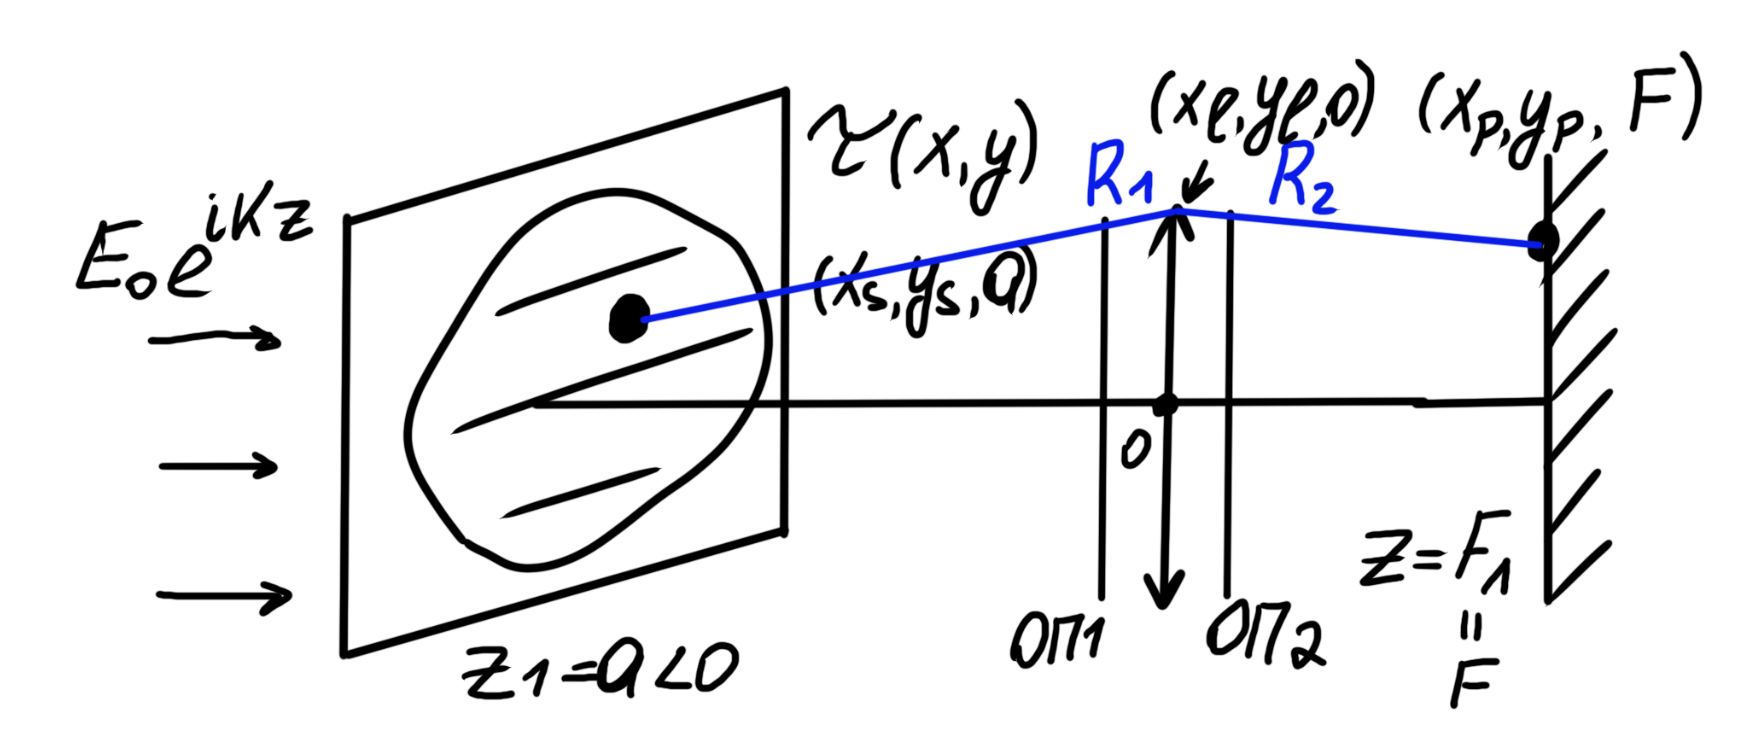
\includegraphics[width=0.7\textwidth]{/Users/vladbelousov/Desktop/Semestr_4-FP-NSU/ЭиО/Лекции_по_дням/image/174.png}
\end{center}

Если \( \displaystyle  \frac{1}{a }  + \frac{1}{F }  = \frac{1}{b}  \), то на экране: 

\begin{center}
    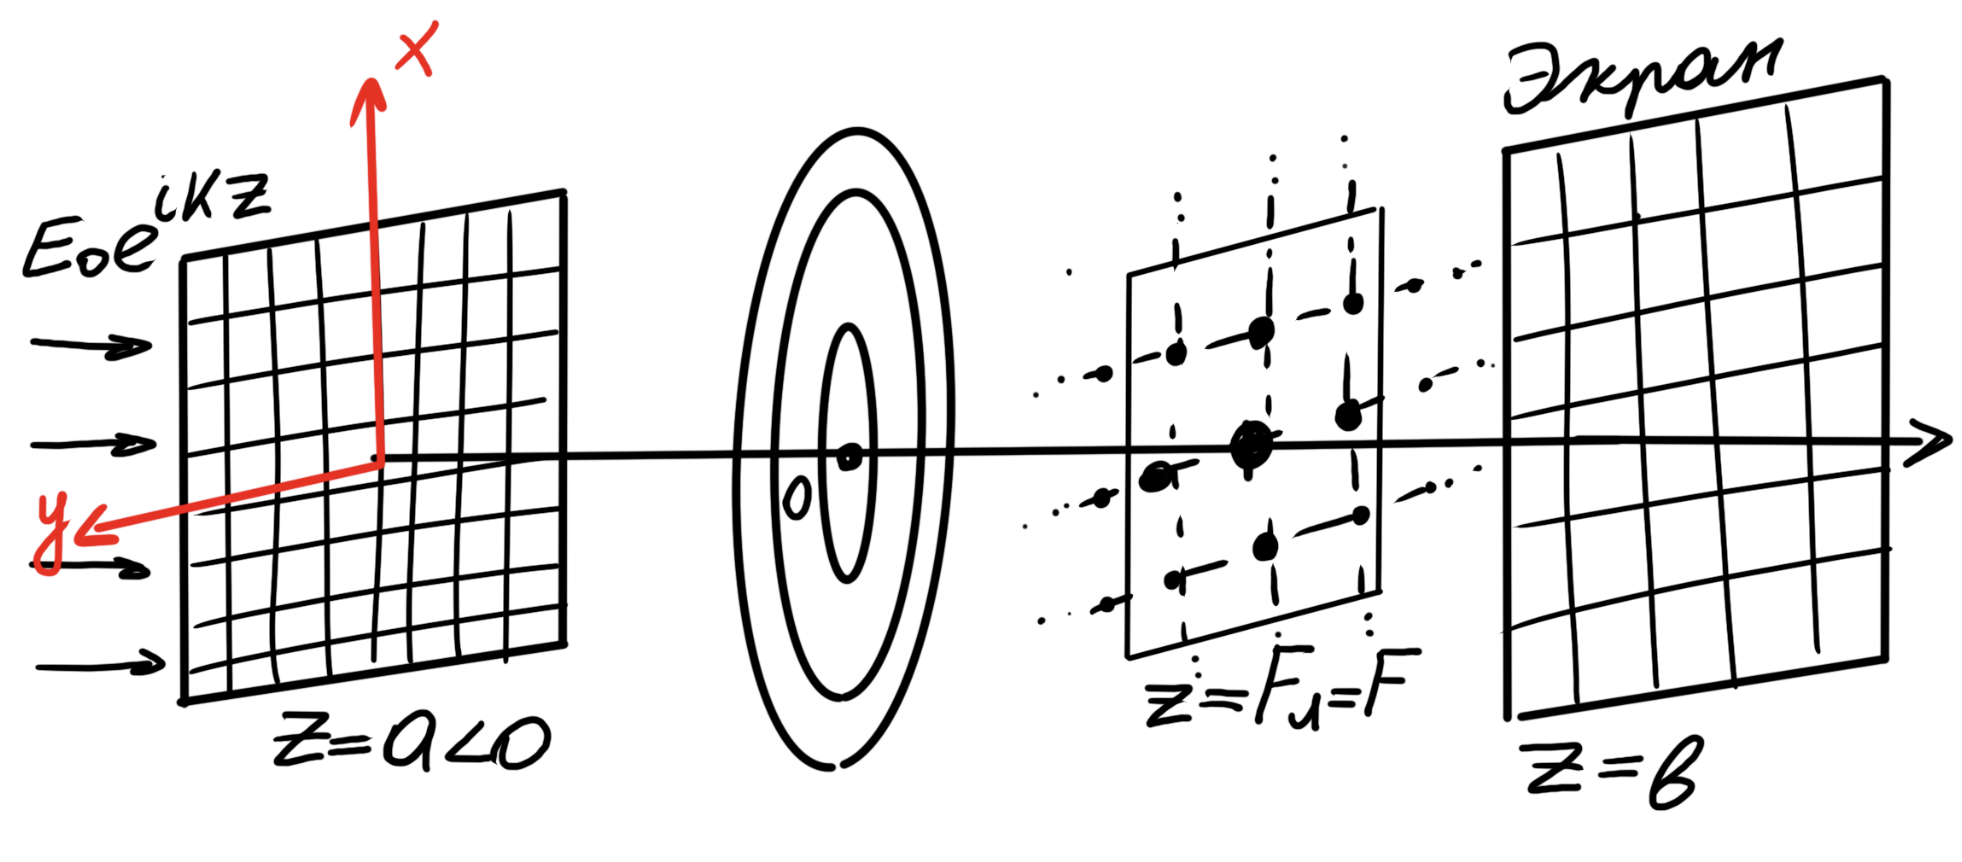
\includegraphics[width=0.7\textwidth]{/Users/vladbelousov/Desktop/Semestr_4-FP-NSU/ЭиО/Лекции_по_дням/image/175.png}
\end{center}


\begin{center}
    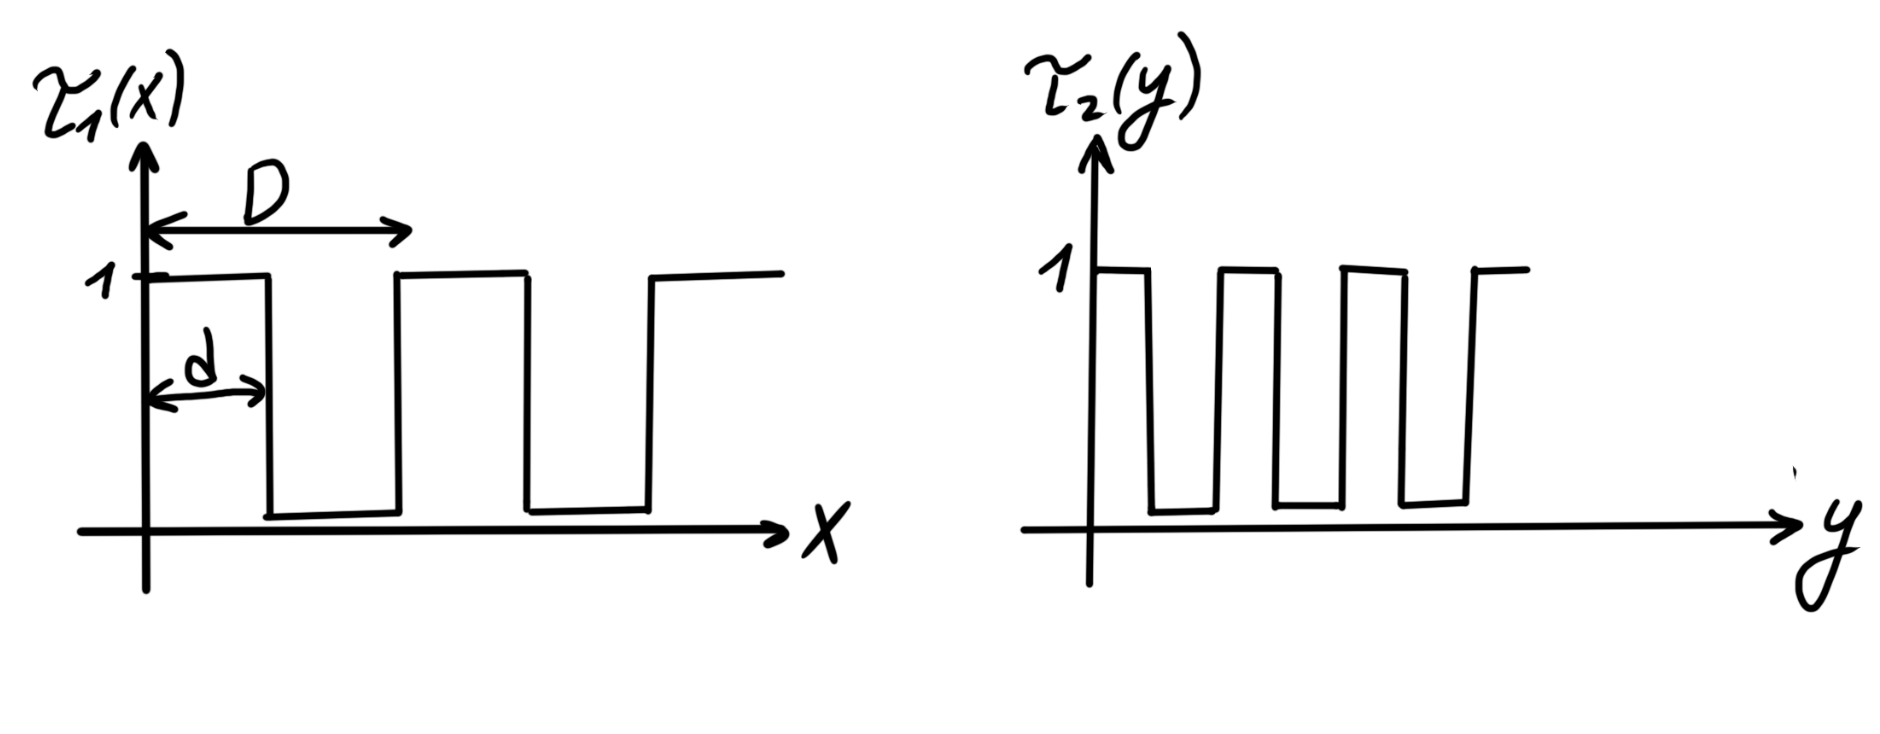
\includegraphics[width=0.7\textwidth]{/Users/vladbelousov/Desktop/Semestr_4-FP-NSU/ЭиО/Лекции_по_дням/image/176.png}
\end{center}
\( \tau (x,y ) = \tau_1 (x) \cdot \tau_2 (y) \) 

\[ \hat{ \tau } (k_x , k_y ) = \frac{1}{2 \pi } \int_{-\infty}^{\infty}  \tau_1 (x ) e^{ - i k_x x } dx \int_{-\infty}^{\infty} \tau_2 (y ) e^{ - i k_y y } dy = \hat{ \tau } _1 (k_x ) \hat{ \tau }_2 (k_y)       \] 

В фокальной плоскости линзы выполнено условие для дифракции Фраунгофера. 


\[ \hat{ E }  (k_x ) = \mathrm{sinc }  ^2 \left(  \frac{kd}{2 }  \left(  \sin \theta_0 - \sin \theta  \right) \right)  \frac{\displaystyle  \sin  ^2 \left( \frac{NkD}{2 }  \left( \sin \theta_0 - \sin \theta \right) \right)}{\displaystyle \sin  ^2 \left( \frac{kD}{2 }  \left(  \sin \theta_0 - \sin \theta \right) \right)}  \] 
, где \( \sin \theta_0 = 0 \) 

\begin{center}
    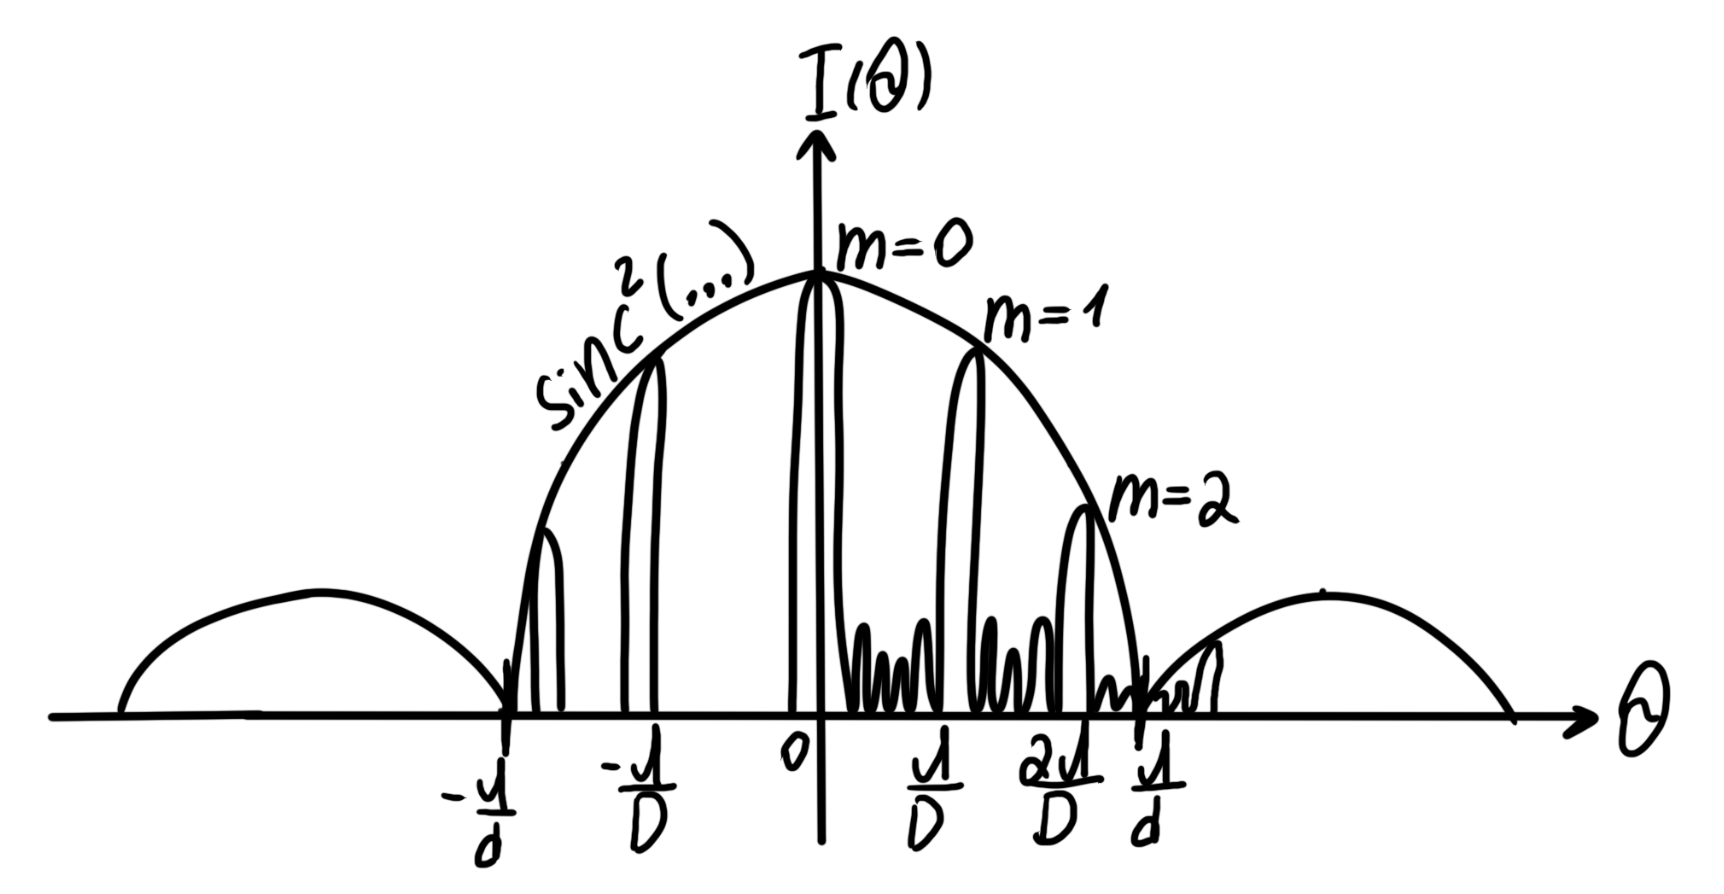
\includegraphics[width=0.7\textwidth]{/Users/vladbelousov/Desktop/Semestr_4-FP-NSU/ЭиО/Лекции_по_дням/image/177.png}
\end{center}

Главные максимумы \( \displaystyle  \frac{kD}{2 }  \sin \theta_m = \pi m \Rightarrow \sin \theta_m \approx \theta_m = m \frac{\lambda}{D }  \) 

%%-------------------------------%%

% Закрытие документа, если файл компилируется отдельно
\ifdefined\mainfile
    % Если это основной файл, не нужно заканчивать документ
\else
    \end{document}
\fi